\documentclass[12pt,a4paper]{article}

% ============================================================
% PACKAGES
% ============================================================
\usepackage[
    a4paper,
    top=1.55cm,
    bottom=1.35cm,
    left=1.75cm,
    right=1.75cm
]{geometry}

\usepackage[T1]{fontenc}
\usepackage{newtxtext}
\usepackage{graphicx}
\usepackage{xcolor}
\usepackage{array}
\usepackage{tabularx}
\usepackage{fancyhdr}
\usepackage{tikz}
\usepackage{eso-pic}
\usepackage{ragged2e}

% ============================================================
% COLORS
% ============================================================
\definecolor{GEUBlue}{RGB}{43,91,145}
\definecolor{GEUBannerBlue}{RGB}{0,102,148}
\definecolor{GEUYellow}{RGB}{255,201,38}
\definecolor{InstructionGrey}{RGB}{125,125,125}

% ============================================================
% GENERAL SETTINGS
% ============================================================
\setlength{\parindent}{0pt}
\setlength{\parskip}{0pt}
\renewcommand{\arraystretch}{1}

% ============================================================
% HEADER / FOOTER
% ============================================================
\pagestyle{fancy}
\fancyhf{}

\fancyhead[L]{%
    \fontsize{10.5}{12}\selectfont
    COURSE NAME AND ID
}

\fancyhead[R]{%
    \fontsize{10.5}{12}\selectfont
    PHASE-II PROJECT PROGRESS
}

\fancyfoot[R]{%
    \fontsize{10}{12}\selectfont
    Page \thepage
}

\renewcommand{\headrulewidth}{0pt}
\renewcommand{\footrulewidth}{0pt}

\setlength{\headheight}{20pt}
\setlength{\headsep}{0.65cm}
\setlength{\footskip}{0.65cm}

% ============================================================
% BOTTOM YELLOW LINE
% ============================================================
\AddToShipoutPictureBG{%
\begin{tikzpicture}[remember picture,overlay]
    \fill[GEUYellow]
    (current page.south west)
    rectangle
    ([yshift=0.14cm]current page.south east);
\end{tikzpicture}
}

% ============================================================
% CUSTOM COMMANDS
% ============================================================
\newcommand{\sectiontitle}[1]{%
    {\color{GEUBlue}
    \fontsize{18}{22}\selectfont #1}
}

\newcommand{\instruction}[1]{%
    {\color{InstructionGrey}
    \fontsize{10.5}{13}\selectfont #1}
}

\newcommand{\answerbox}[2]{%
    \begin{tabularx}{\textwidth}{
        |>{\raggedright\arraybackslash}X|}
        \hline
        \parbox[t][#1][t]{\dimexpr\linewidth-12pt\relax}{
            \vspace{5pt}
            \fontsize{11}{13}\selectfont #2
        }\\
        \hline
    \end{tabularx}
}

% ============================================================
% DOCUMENT
% ============================================================
\begin{document}

% ============================================================
% PAGE 1
% ============================================================

\vspace*{0.10cm}

% Upload Graphic Era logo as graphicera_logo.png

\includegraphics[width=8.0cm]{geulogo.png}

\vspace{0.70cm}

\noindent
\colorbox{GEUBannerBlue}{%
\parbox{\dimexpr\textwidth-2\fboxsep\relax}{
    \vspace{0.17cm}
    {\color{GEUYellow}
    \fontsize{16.5}{20}\selectfont
    \bfseries
    PROJECT AND TEAM INFORMATION}
    \vspace{0.17cm}
}}

\vspace{0.80cm}

% PROJECT TITLE
\sectiontitle{Project Title}

\vspace{0.05cm}

\instruction{(Try to choose a catchy title. Max 20 words).}

\vspace{0.40cm}

\answerbox{1.00cm}{NestInvest: A Secure Web Desk for Stock Tracking, Comparison, and Technical Forecast}

\vspace{0.80cm}

% STUDENT INFORMATION
% \sectiontitle{Student/Team Information}

% \vspace{0.40cm}

% \begin{tabularx}{\textwidth}{
% |>{\raggedright\arraybackslash}p{0.66\textwidth}
% |>{\raggedright\arraybackslash}X|
% }
% \hline

% \parbox[t][1.15cm][t]{\linewidth}{
% \vspace{4pt}
% \fontsize{10.5}{13}\selectfont
% Team Name:\\[2pt]
% Team \# (Mentor needs to assign)
% }
% &
% \\
% \hline

% \parbox[t][3.65cm][t]{\linewidth}{
% \vspace{5pt}
% \fontsize{10.5}{13}\selectfont
% Team member 1 (Team Lead)\\[3pt]
% {\color{InstructionGrey}
% (Last Name, name: student ID: email, picture):}
% }
% &
% \\
% \hline

% \parbox[t][3.65cm][t]{\linewidth}{
% \vspace{5pt}
% \fontsize{10.5}{13}\selectfont
% Team member 2\\[3pt]
% {\color{InstructionGrey}
% (Last Name, name: student ID: email, picture):}
% }
% &
% \\
% \hline

% \end{tabularx}

% \newpage
\noindent
\begin{tabularx}{\textwidth}{|>{\RaggedRight\arraybackslash}p{0.69\textwidth}|>{\RaggedRight\arraybackslash}X|}
\hline
\begin{minipage}[t]{\linewidth}
\vspace{1.5mm}
\textit{Team Name:}\\[-1mm]
\textit{Team \#}
\vspace{1.5mm}
\end{minipage}
&
\begin{minipage}[t]{\linewidth}
\vspace{1.5mm}
\textit{NestInvest}\\
\textit{[Fill official team number]}
\vspace{1.5mm}
\end{minipage}
\\
\hline
\begin{minipage}[t][3.25cm][t]{\linewidth}
\vspace{1.5mm}
\textbf{Team member 1 (Team Lead)}\\[-1mm]
\textit{(Last Name, name: student ID: email, picture):}
\vspace{2.0cm}
\end{minipage}
&
\begin{minipage}[t][3.25cm][t]{\linewidth}
\vspace{1.5mm}
\textit{Sharma, Yash -- [Fill student ID]}\\
\textit{[Fill email]}\\
\textit{B.Tech CSE, Graphic Era Deemed to be University, Dehradun}

\vspace{2mm}
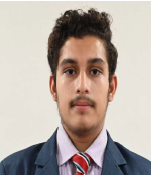
\includegraphics[width=3.0cm,height=1.5cm,keepaspectratio]{member1.png}
\end{minipage}
\\
\hline
\begin{minipage}[t][3.25cm][t]{\linewidth}
\vspace{1.5mm}
\textbf{Team member 2}\\[-1mm]
\textit{(Last Name, name: student ID: email, picture):}
\vspace{2.0cm}
\end{minipage}
&
\begin{minipage}[t][3.25cm][t]{\linewidth}
\vspace{1.5mm}
\textit{Rawat, Yashraj -- [Fill student ID]}\\
\textit{[Fill email]}\\
\textit{B.Tech CSE, Graphic Era Deemed to be University, Dehradun}

\vspace{2mm}
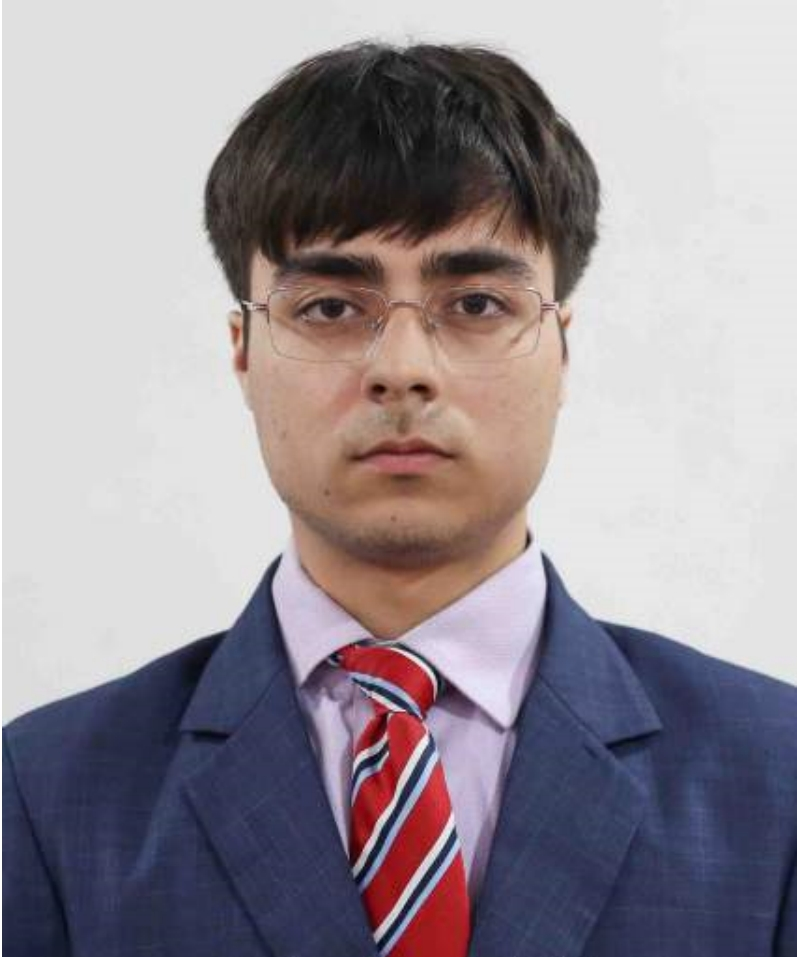
\includegraphics[width=3.0cm,height=1.5cm,keepaspectratio]{member2.png}
\end{minipage}
\\
\hline
\begin{minipage}[t][3.25cm][t]{\linewidth}
\vspace{1.5mm}
\textbf{Team member 3}\\[-1mm]
\textit{(Last Name, name: student ID: email, picture):}
\vspace{2.0cm}
\end{minipage}
&
\begin{minipage}[t][3.25cm][t]{\linewidth}
\vspace{1.5mm}
\textit{Rana, Vivek -- [Fill student ID]}\\
\textit{[Fill email]}\\
\textit{B.Tech CSE, Graphic Era Deemed to be University, Dehradun}

\vspace{2mm}
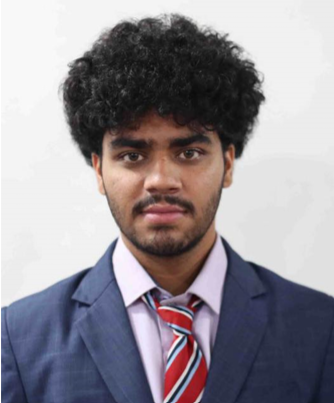
\includegraphics[width=3.0cm,height=1.5cm,keepaspectratio]{member3.png}
\end{minipage}
\\
\hline
\begin{minipage}[t][3.25cm][t]{\linewidth}
\vspace{1.5mm}
\textbf{Team member 4}\\[-1mm]
\textit{(Last Name, name: student ID: email, picture):}
\vspace{2.0cm}
\end{minipage}
&
\begin{minipage}[t][3.25cm][t]{\linewidth}
\vspace{1.5mm}
\textit{Not applicable. The team has three members.}

\vspace{2mm}
 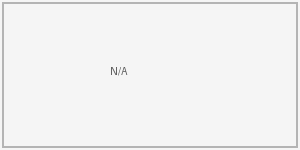
\includegraphics[width=3.0cm,height=1.5cm,keepaspectratio]{member4.png}
\end{minipage}
\\
\hline
\end{tabularx}

\newpage
% ============================================================
% PAGE 2
% ============================================================

\vspace*{0.15cm}

\noindent
\colorbox{GEUBannerBlue}{%
\parbox{\dimexpr\textwidth-2\fboxsep\relax}{
    \vspace{0.18cm}
    {\color{GEUYellow}
    \fontsize{17}{21}\selectfont
    \bfseries
    PHASE-II PROJECT PROGRESS DESCRIPTION (35 pts)}
    \vspace{0.18cm}
}}

\vspace{0.70cm}

% PROJECT ABSTRACT
\sectiontitle{Project Abstract (2 pts)}

\vspace{0.05cm}

\instruction{
(Brief restatement of your project's main goal. Max 300 words).
}

\vspace{0.12cm}

\answerbox{3.60cm}{NestInvest is a web stock desk built at Graphic Era Deemed to be University, Dehradun. It grew from a console app that fetched quotes, profiles, and news. Phase II is a responsive dashboard (``hatch, hold, grow''). A registered user can search a symbol, view 1D--1Y charts, keep a watchlist, track a portfolio, compare stocks, read news, set alerts, and see a technical forecast. Login uses email and password, Google, and X, with hashed passwords and sessions. Market data comes from Yahoo-style endpoints. The project shows web architecture, security, data structures, and object-oriented design. It is not investment advice.}

\vspace{0.70cm}

% UPDATED PROJECT APPROACH
\sectiontitle{Updated Project Approach and Architecture (2 pts)}

\vspace{0.05cm}

\instruction{
(Describe your current approach, including system design,
communication protocols, libraries used, etc.\\
Max 300 words).
}

\vspace{0.25cm}

\answerbox{4.75cm}{Client--server app. React and Tailwind in the browser; TanStack Start over HTTPS; TanStack Query for quotes; Zustand for watchlist, portfolio, alerts, and theme; Recharts for charts. PostgreSQL (Neon, or PGLite in preview). Better Auth: hashed passwords, HttpOnly cookies. Product routes reject guests and platform viewer identities.\\[2pt]
\textbf{OOP.} Candle, Forecast, Holding, and PriceAlert encapsulate state. Indicators share one vote interface (abstraction and polymorphism). Auth, mail, rate limiting, and roles are separate modules.\\[2pt]
\textbf{DSA.} Price history is an array. SMA, EMA, and RSI use a sliding window. The watchlist is a hash map for O(1) lookup. Chart ranges use binary search on sorted times. Recent symbols are a capped stack. Alerts use a min-heap. Portfolio ranking is a comparison sort. Tokens are stored as SHA-256 digests and looked up in a hash table.}

\newpage

% ============================================================
% PAGE 3
% ============================================================

\vspace*{0.20cm}

% TASKS COMPLETED
\sectiontitle{Tasks Completed (7 pts)}

\vspace{0.05cm}

\instruction{
(Describe the main tasks that have been assigned and already completed.
Max 250 words).
}

\vspace{0.20cm}

\begin{tabularx}{\textwidth}{
|>{\raggedright\arraybackslash}X
|>{\raggedright\arraybackslash}X|
}
\hline
\textbf{Task Completed} &
\textbf{Team Member}\\
\hline

\parbox[t][3.25cm][t]{\linewidth}{\vspace{2pt}\fontsize{8.5}{10}\selectfont
Console review and web design for NestInvest\\
Branding: name, logo lockup, team footer\\
Chart ranges (1D--1Y) and news cards\\
Watchlist, portfolio, comparison, market overview\\
Dark/light theme and mobile layout\\
Auth: signup, login, logout, verify, reset, sessions\\
Technical forecast: SMA, EMA, RSI, MACD, Bollinger\\
DSA and OOP design mapped onto the features}
&
\parbox[t][3.25cm][t]{\linewidth}{\vspace{2pt}\fontsize{8.5}{10}\selectfont
Sharma, Yash\\
Sharma, Yash\\
Rawat, Yashraj\\
Rana, Vivek\\
Rawat, Yashraj\\
Sharma, Yash\\
Rana, Vivek\\
All three}
\\
\hline
\end{tabularx}

\vspace{0.65cm}

% CHALLENGES
\sectiontitle{Challenges/Roadblocks (7 pts)}

\vspace{0.05cm}

\instruction{
(Describe the challenges that you have faced or are facing so far
and how you plan to solve them. Max 300 words).
}

\vspace{0.18cm}

\answerbox{4.05cm}{Four issues shaped Phase II. The preview can mint a platform viewer identity; product routes now require a real registered email and reject that viewer. The console used Finnhub; the web app uses Yahoo-style endpoints so keys stay off the browser. Caching and an empty state will cover missing fields. Real mail needs EMAIL\_API\_KEY; without it, preview can show a one-time link only. Facebook is not on the allowed broker, so social login is Google and X. The DSA design is fixed. The named modules (hash map, binary search, min-heap, stack) still need to be wired so the running code matches this report.}

\vspace{0.65cm}

% TASKS PENDING
\sectiontitle{Tasks Pending (7 pts)}

\vspace{0.05cm}

\instruction{
(Describe the main tasks that you still need to complete.
Max 250 words).
}

\vspace{0.18cm}

\begin{tabularx}{\textwidth}{
|>{\raggedright\arraybackslash}X
|>{\raggedright\arraybackslash}X|
}
\hline

\textbf{Task Pending} &
\textbf{Team Member (to complete the task)}
\\
\hline

\parbox[t][1.25cm][t]{\linewidth}{\vspace{1pt}\fontsize{8}{9.5}\selectfont
Named DSA modules: map, binary search, heap, stack\\
Class diagram and indicator wrappers for the viva\\
Production mail, admin allowlist, demo, fill IDs and repo URL}
&
\parbox[t][1.25cm][t]{\linewidth}{\vspace{1pt}\fontsize{8}{9.5}\selectfont
Sharma, Yash\\
Rawat, Yashraj\\
Sharma / Rana / All three}
\\
\hline

\end{tabularx}

\newpage

% ============================================================
% PAGE 4
% ============================================================

\vspace*{0.30cm}

% PROJECT OUTCOME
\sectiontitle{Project Outcome/Deliverables (2 pts)}

\vspace{0.05cm}

\instruction{
(Describe what are the key outcomes / deliverables of the project.
Max 200 words).
}

\vspace{0.35cm}

\answerbox{3.35cm}{The key deliverable is a working NestInvest desk. A user can register, verify, sign in, and reach a protected dashboard. The desk has an interactive chart, watchlist, portfolio with cost and profit or loss, market overview, stock comparison, news cards, dark and light mode, a mobile layout, and price alerts. A technical forecast uses moving averages, RSI, MACD, and Bollinger bands. Authentication uses hashed passwords and server-side checks. DSA and OOP are mapped to these features. Supporting deliverables are the source, database migrations, this report, and a short demo.}

\vspace{0.75cm}

% PROGRESS OVERVIEW
\sectiontitle{Progress Overview (2 pts)}

\vspace{0.05cm}

\instruction{
(Summarize how much of the project is done, what's behind schedule,
what's ahead of schedule. Max 200 words.)
}

\vspace{0.25cm}

\answerbox{4.45cm}{About three quarters of Phase II is done. Branding, the nine desk features, the technical forecast, and authentication are ahead of a typical mid-phase checkpoint. The named data-structure modules and production mail are slightly behind: the design is finished, the code is not fully separated into the structures named here. Filling student IDs, the course code, the team number, and the repository link is administrative and can be done in one sitting. If the DSA modules are coded this week, the team is on track for the Phase-II evaluation.}

\newpage

% ============================================================
% PAGE 5
% ============================================================

\vspace*{0.20cm}

% CODEBASE
\sectiontitle{Codebase Information (2 pts)}

\vspace{0.05cm}

\instruction{
(Repository link, branch, and information about important commits.)
}

\vspace{0.20cm}

\answerbox{3.70cm}{Repository: [Fill GitHub or university repository URL]\\
Branch: main\\[2pt]
Important work already in the tree: NestInvest desk (chart ranges, watchlist, portfolio, comparison, news, alerts, theme); forecast module with sliding-window indicators; Better Auth for email and password, Google, and X, plus verification, reset, sessions, and roles; database migrations for the user profile, hashed tokens, and rate-limit attempts.\\[2pt]
Replace the URL and add two or three real commit messages before submission.}

\vspace{0.65cm}

% TESTING
\sectiontitle{Testing and Validation Status (2 pts)}

\vspace{0.05cm}

\instruction{(Provide information about any tests conducted)}

\vspace{0.30cm}

\begin{tabularx}{\textwidth}{
|>{\raggedright\arraybackslash}p{0.34\textwidth}
|>{\raggedright\arraybackslash}p{0.31\textwidth}
|>{\raggedright\arraybackslash}X|
}
\hline

\textbf{Test Type} &
\textbf{Status (Pass/Fail)} &
\textbf{Notes}
\\
\hline

\parbox[t][1.20cm][t]{\linewidth}{\vspace{1pt}\fontsize{8}{9.5}\selectfont
Password, rate limit, viewer identity, token single-use, typecheck, CSRF origin, cookie flags, manual UI}
&
\parbox[t][1.20cm][t]{\linewidth}{\vspace{1pt}\fontsize{8}{9.5}\selectfont
Pass\\[2pt]
Live email and admin path: Pending}
&
\parbox[t][1.20cm][t]{\linewidth}{\vspace{1pt}\fontsize{8}{9.5}\selectfont
Unit tests and a live login check. HttpOnly, Secure, SameSite=Lax. Email needs EMAIL\_API\_KEY; admin needs ADMIN\_EMAILS.}
\\
\hline

\end{tabularx}

\vspace{0.65cm}

% DELIVERABLES PROGRESS
\sectiontitle{Deliverables Progress (2 pts)}

\vspace{0.05cm}

\instruction{
(Summarize the current status of all key project deliverables
mentioned earlier. Indicate whether each deliverable is completed,
in progress, or pending.)
}

\vspace{0.25cm}

\answerbox{3.20cm}{Working NestInvest application --- completed. Nine desk features and technical forecast --- completed. Authentication and authorization --- completed. DSA and OOP design mapped to features --- completed. Named DSA modules in code --- in progress. Production email --- pending (external key). This Phase-II report --- in progress (personal fields still to fill). Demo script and screenshots --- pending.}

\end{document}
